
Este año los ganadores del Premio Nobel de Fisica ha sido otorgado a
\emph{Isamu Akasaki}, \emph{Hiroshi Amano} y \emph{Shuji Nakamura} por
su desarrollo en LED's azules eficientes.

Hace ya años que el LED lo encontramos en nuestro entorno: pantallas
de los teléfonos inteligentes, tablets, ordenadores y televisores,
coches y bombillas de los hogares. Las principales caracterísitcas de
los LEDs es que son más duraderos, baratos, pequeños y eficientes con
hasta 300 lumen/watio a los 70 de los fluorescentes y 16 de las
bombillas tradicionales. Vamos a explicaros las características del
invento merecedor de este Nobel.


\section{Qué es un LED}

El LED, acrónimo de ''Light Emitting Diode”, o diodo emisor de luz de
estado sólido constituye un tipo especial de
semiconductor, cuya característica principal es convertir en luz la
corriente eléctrica de bajo voltaje que atraviesa su chip. Desde el
punto de vista físico un LED común se presenta como un bulbo
miniaturizado, carente de filamento o de cualquier otro tipo de
elemento o material peligroso, con la ventaja sobre otras tecnologías
que no contamina el medio ambiente.

Los LEDs son unos diodos especiales que emiten luz cuando pasa
corriente en la dirección permitida. Esta emisión de luz se produce
por un salto de los electrones entre niveles de energía y deben
cumplirse unas propiedas para que exista y podamos ver esa luz. En
concreto tienen que cumplirse dos condiciones sencillas, la primera de
las cuales es que el mínimo de un nivel de energía se encuentre justo
encima del máximo del nivel anterior. Estos semiconductores se llaman
de “gap directo” (gap es la diferencia de energías). La segunda
condición es que el gap de energía entre un nivel y otro sea tal que
el fotón resultante tenga una frecuencia en el rango visible. Es
decir, el gap debe de ser del tamaño justo para poder ver la luz y que
no sea infrarroja (gap pequeño) o ultravioleta (gap
grande). Modificando el tamaño del gap podemos variar el color desde
el rojo hasta el azul pasando por todos los del arcoiris.


\section{Problemáticas con los LEDs}
Si aumentamos mucho el gap (por encima del color verde) es más fácil
perder las propiedades de semiconductor y pasar a un aislante
convencional como el cuarzo o el vidrio. Aquí es donde reside la
dificultad de conseguir un LED azul: aumentar el gap lo suficiente
manteniendo un semiconductor. Como veremos a continuación esto no es
sencillo y costó mucho tiempo y dinero conseguirlo de una forma viable
para la producción masiva. Y esta es una de la razones de este
merecido Nobel de fíusica sobre Led azul eficiente.

\section{Evolución del LED}

El primer LED fue con emisión en rojo y fue construido en 1962. Aunque
ya antes se habían observado fenómenos similares en el
infrarrojo. Desde entonces se mantuvo una carrera por conseguir el
resto de colores. A pesar de tenerse los diseños desde los años 50 el
LED azul aún se haría esperar varias décadas. Sobre 1970 la mejora en
las técnicas de crecimiento de cristales permitió un gran avance en el
desarrollo de nuestros queridos LEDs azules. En principio se
intentaron basar en GaN (Nitruro de Galio) pero pronto se vio que esa
técnica no conseguía una luminosidad suficiente. Es aquí donde podemos
establecer la creación del primer LED azul, aunque no era usable y
apenas se veía su luz. Fue en 1989 como la fecha en que se consiguió
el primer LED azul con una emisión razonablemente alta, aunque su
eficiencia era del 0.03\%.  Una vez más parecía que el LED azul no era
viable para la producción masiva; hasta que en 1994 los ganadores de
este Nobel de Física obtuvieron por primera vez un LED azul de “alta”
eficiencia utilizando técnicas modernas. Como semiconductor usaron
InGaN/AlGaN y obtuvieron eficiencia alrededor de 2.7\% (comparable al
4\% de las bombillas incandescentes).

A día de hoy los LEDs corrientes que podemos comprar en cualquier
tienda, muy baratos, tienen una eficiencia superior al 50\% y
presentan la mejor fuente de luz artificial que conocemos. El LED azul
{\bf eficiente} ha permitido, en primer
lugar, completar las matrices RGB que usan hoy todas las pancartas LED
del mundo así como obtener LEDs blancos.

\begin{center}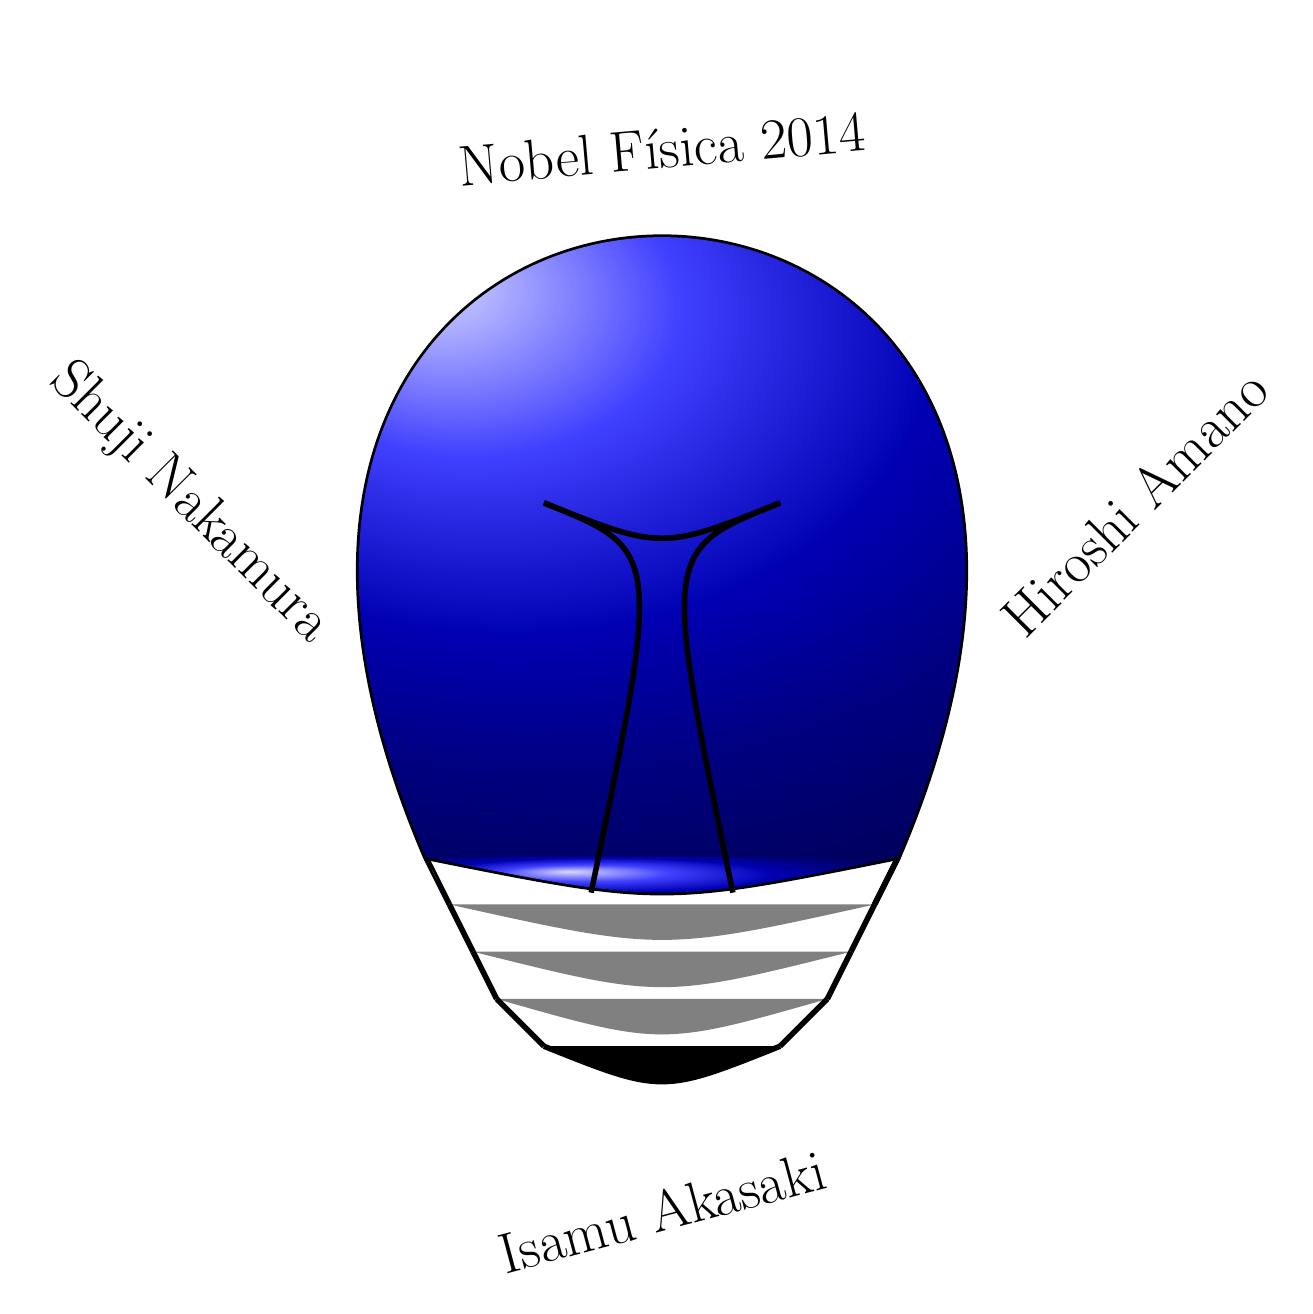
\begin{tikzpicture}[line width=2pt,scale=3]
\draw (-1,0) .. controls (-2.5,3.5) and (2.5,3.5) .. (1,0);
\draw (-1,0) .. controls (0,-0.2) .. (1,0);
\draw (-1,0)--(-0.9,-0.2);\draw (1,0)--(0.9,-0.2);
\shade[shading=ball, ball color=blue] (-1,0) .. controls (-2.5,3.5) and (2.5,3.5) .. (1,0);
\shade[shading=ball, ball color=blue] (-1,0) .. controls (0,-0.2) .. (1,0);
\shade[shading=ball, ball color=blue] (-1,0)--(-0.9,-0.2);\draw (1,0)--(0.9,-0.2);
\fill[color=gray] (-0.9,-0.2) .. controls (0,-0.4) .. (0.9,-0.2);
\draw (-0.9,-0.2)--(-0.8,-0.4);\draw (0.9,-0.2)--(0.8,-0.4);
\fill[color=gray] (-0.8,-0.4) .. controls (0,-0.6) .. (0.8,-0.4);
\draw (-0.8,-0.4)--(-0.7,-0.6);\draw (0.8,-0.4)--(0.7,-0.6);
\fill[color=gray] (-0.7,-0.6) .. controls (0,-0.8) .. (0.7,-0.6);
\draw (-0.7,-0.6)--(-0.5,-0.8);\draw (0.7,-0.6)--(0.5,-0.8);
\fill[color=black] (-0.5,-0.8) .. controls (0,-1) .. (0.5,-0.8);
\draw (-0.5,-0.8) .. controls (0,-1) .. (0.5,-0.8);
\draw (-0.3,-0.15)..controls (0,1.3) .. (-0.5,1.5);
\draw (0.3,-0.15)..controls (0,1.3) .. (0.5,1.5);
\draw (0.5,1.5)..controls (0,1.3) .. (-0.5,1.5);
\coordinate (P1) at (0,-1.5);
\draw (P1) node[rotate=15] (N) {\huge{Isamu Akasaki}};
\coordinate (P1) at (2,1.5);
\draw (P1) node[rotate=45] (N) {\huge{Hiroshi Amano}};
\coordinate (P1) at (-2,1.5);
\draw (P1) node[rotate=-45] (N) {\huge{Shuji Nakamura}};
\coordinate (P1) at (0,3);
\draw (P1) node[rotate=5] (N) {\huge{Nobel Física 2014}};
\end{tikzpicture}
\end{center}


\newpage

%%% Local Variables: 
%%% mode: latex
%%% TeX-master: "novedades"
%%% End: 



